\section{Auswertung}
\label{sec:Auswertung}
\subsection{Graphische Visualisierung}
\begin{figure}
  \centering
  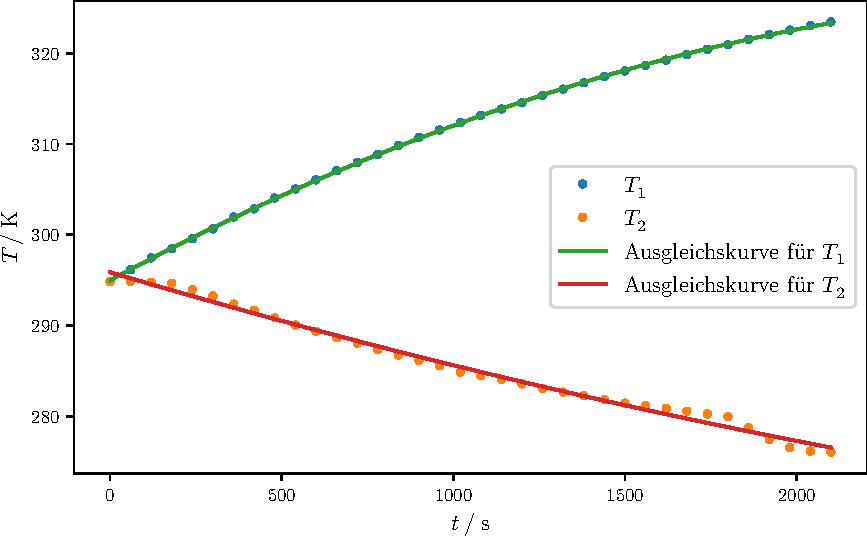
\includegraphics{temperatur.pdf}
  \caption{Temperaturverleif beider Reservoirs.}
  \label{fig:temperatur}
\end{figure}
\subsection{Nicht-lineare Ausgleichsrechnung}
Der nicht-lineare Zusammenhang zwischen der Zeit und der Temperatur lässt sich mittels einer quadtratischen Ausgleichskurve, welche durch 
\begin{equation}
  T(t) = At^2 + Bt + C
\end{equation}
beschrieben wird, approximieren. Mittels Rechnungen in Python ergaben sich die Ausgleichskfunktionen zu
\begin{align}
  T_1(t) &= - 0.0116t^2 + 1.2168 t + 294.7008 \\
  T_2(t) &= \phantom{-}  0.0034 t^2 - 0.6725 t + 295.8702
\end{align}
\subsection{Differentialquotient}
Der Differentialquotienten von $T_1(t)$ und $T_2(t)$ sind durch
\begin{align}
  \frac{\symup{d} T_1(t)}{\symup{d}t} = - 0.0232t + 1.2168  \\
  \frac{\symup{d} T_2(t)}{\symup{d}t} = \phantom{-} 0.0068 t - 0.6725 
\end{align}
gegeben. Die in die Differentialquotienten eingesetzen Zeitpunkte $t = 10$, $t = 15$, $t = 20$ und $t = 35$ ergeben folgende Tabelle:
\begin{table}
  \centering
  \caption{Ergebnisse der Differentialquotienten}
  \label{tab:TabelleDifferentialquotient}
  \sisetup{table-format = 1.4}
  \begin{tabular}{S[table-format = 2.0] S S}
    \toprule
    {$t \mathbin{/} \si{\minute}$} & {$\frac{\symup{d} T_1(t)}{\symup{d}t} \mathbin{/} \si{\kelvin\minute\tothe{-1}}$} & 
    {$\frac{\symup{d} T_2(t)}{\symup{d}t} \mathbin{/} \si{\kelvin\minute\tothe{-1}}$} \\
    \midrule
    10 & 0.9848 &-0.6045 \\
    15 & 0.8688 &-0.5705 \\
    20 & 0.7528 &-0.5365 \\
    35 & 0.4048 &-0.4345 \\
    \bottomrule                         
  \end{tabular}
\end{table}